\documentclass[12pt,a4paper]{article}
\usepackage[margin=2.5cm]{geometry}
\usepackage{amsmath,amssymb,amsthm}
\usepackage{graphicx}
\usepackage{booktabs}
\usepackage{hyperref}
\usepackage{xcolor}
\usepackage{algorithm}
\usepackage{algpseudocode}
\usepackage{cite}
\usepackage{float}
\usepackage{caption}
\usepackage{subcaption}
\usepackage{tikz}
\usetikzlibrary{shapes.geometric, arrows, positioning, fit, backgrounds}

\hypersetup{
    colorlinks=true,
    linkcolor=blue!70!black,
    citecolor=green!50!black,
    urlcolor=blue!70!black,
}

\title{\textbf{Task 3.2: Secure, Privacy-Preserved and Incentive-Based\\
Data Sharing in UAV Networks for Emergency Response}\\[6pt]
\large COVER Project --- EU MSCA Staff Exchanges, Grant No.\ 101086228}

\author{Henry Kabuye\\
\small Northumbria University\\
\small Supervisor: Professor Nauman Aslam\\
\small COVER Project --- Task 3.2 (Lead: Georg-August-Universit\"at G\"ottingen)\\
\small Supported by: CentraleSupelec (CS) and UESTC}

\date{May 2026}

\begin{document}

\maketitle
\begin{abstract}
This report presents the design and simulation of a comprehensive data-sharing
framework for cooperative UAV networks in emergency response scenarios, developed
under Task 3.2 of the COVER project.  The framework integrates five tightly coupled
components: (i)~a blockchain-based security layer using Proof-of-Authority (PoA)
consensus to defend against Sybil, Byzantine, and free-rider attacks;
(ii)~a Stackelberg game-theoretic incentive mechanism with Proof-of-Resource-Sharing
(PoRS) that elicits truthful participation from heterogeneous UAV agents;
(iii)~Differentially Private Stochastic Gradient Descent (DP-SGD) with tight Rényi
Differential Privacy (RDP) accounting for gradient privacy;
(iv)~Federated Learning (FL) with convergence analysis under 3D UAV mobility and
bandwidth-limited wireless channels; and (v)~a \emph{Multi-Agent Reinforcement
Learning (MARL) agentic framework} in which each UAV independently learns an
adaptive participation policy via Deep Q-Networks (DQN), with Q-network weights
periodically federated across agents.  All components are implemented in a Python
simulation framework supporting multi-GPU parallelism across three NVIDIA GTX 1070 Ti
GPUs, with DP-SGD accelerated via vectorised per-sample gradients
(\texttt{torch.func.vmap}).  Evaluation uses CIFAR-10 and EuroSAT as proxies for
UAV aerial image classification.
\end{abstract}

\tableofcontents
\newpage

%----------------------------------------------------------------------
\section{Introduction}
%----------------------------------------------------------------------

The COVER project (Cooperative and Intelligent Unmanned Aerial Vehicles for
Emergency Response Applications) aims to develop intelligent, connected UAV
networks capable of supporting first responders in extreme-weather events such as
flooding, wildfires, and earthquakes.  Funded under the Marie Sk\l{}odowska-Curie
Actions Staff Exchanges programme (Grant 101086228), the project runs from
January~2023 to December~2026 with a consortium led by Technische Universiteit
Eindhoven and including Georg-August-Universit\"at G\"ottingen (UGOE, Task 3.2 lead),
CentraleSupelec, KTH, and twelve associated institutions.

Task~3.2 addresses the \emph{data sharing layer}: the mechanisms by which UAVs
collaborate, share sensed data and learned models, while simultaneously maintaining
security against adversaries, protecting the privacy of raw observations, and
providing economic incentives for voluntary resource contribution.

This document describes the methodology, system model, and simulation framework
developed by the author at Northumbria University in the context of Task~3.2,
led by UGOE within the COVER consortium.

%----------------------------------------------------------------------
\section{System Model}
%----------------------------------------------------------------------

\subsection{UAV Network Topology}

We consider $N = 20$ UAVs deployed in a $1000 \times 1000 \times [50,\,200]$~m
three-dimensional operational area.  UAV positions evolve according to the
\emph{3D Random Waypoint Mobility Model}: each UAV selects a waypoint uniformly at
random within the volume, flies at speed $v \sim \mathcal{U}(1, v_{\max})$ with
$v_{\max} = 15$~m/s, pauses for $t_p = 5$~s upon arrival, then repeats.
UAV~0 acts as the parameter server (PS); UAVs~$1,\ldots,N-1$ are worker nodes.

\subsection{Wireless Channel Model}

Air-to-air (A2A) links follow a free-space path loss model with Rician fading:
\begin{equation}
  \mathrm{SNR}_{ij} = P_{\text{tx}} - \mathrm{FSPL}(d_{ij}) + G_{\text{Rician}},
  \label{eq:snr}
\end{equation}
where $\mathrm{FSPL}(d) = 20\log_{10}\!\left(\tfrac{4\pi d f}{c}\right)$,
$f = 5.8$~GHz, and the Rician power gain $G_{\text{Rician}}$ has K-factor
$K = 10$~dB, capturing the dominant line-of-sight component typical in open-sky
UAV operations \cite{alhourani2014}.  A UAV is eligible to participate in an FL
round only if $\mathrm{SNR}_{i,\text{PS}} \geq \gamma_{\min} = 5$~dB.

%----------------------------------------------------------------------
\section{Federated Learning with Differential Privacy (Sub-tasks C \& D)}
%----------------------------------------------------------------------

\subsection{Federated Averaging}

Global model parameters $\mathbf{w}$ are updated via FedAvg \cite{mcmahan2017}:
\begin{equation}
  \mathbf{w}^{(t+1)} = \sum_{k \in \mathcal{S}^{(t)}} \frac{n_k}{N_{\mathcal{S}}}
  \mathbf{w}_k^{(t)},
  \label{eq:fedavg}
\end{equation}
where $\mathcal{S}^{(t)}$ is the set of participating UAVs in round~$t$,
$n_k$ is the number of local samples, and $N_{\mathcal{S}} = \sum_{k\in\mathcal{S}} n_k$.
Each selected UAV runs $E = 5$ local SGD epochs on its private dataset before
uploading the updated weights.

Data heterogeneity across UAVs is modelled via a Dirichlet distribution:
class-conditional indices are split according to
$\mathbf{p}_c \sim \mathrm{Dir}(\alpha \mathbf{1}_N)$ with $\alpha = 0.5$,
producing the non-IID local datasets that are standard in FL research.

\subsection{DP-SGD Local Training}

To prevent the PS from inferring sensitive information from individual model
updates, each participating UAV applies DP-SGD \cite{abadi2016}:

\begin{algorithm}[H]
\caption{DP-SGD at UAV $k$, round $t$}
\begin{algorithmic}[1]
\For{each local epoch $e = 1,\ldots,E$}
  \For{each mini-batch $\mathcal{B} \subset \mathcal{D}_k$}
    \For{each sample $(x_i, y_i) \in \mathcal{B}$}
      \State Compute per-sample gradient $\mathbf{g}_i \leftarrow \nabla_{\mathbf{w}} \ell(\mathbf{w}; x_i, y_i)$
      \State Clip: $\tilde{\mathbf{g}}_i \leftarrow \mathbf{g}_i \cdot \min\!\left(1,\, \tfrac{C}{\|\mathbf{g}_i\|_2}\right)$
    \EndFor
    \State Noise: $\hat{\mathbf{g}} \leftarrow \tfrac{1}{|\mathcal{B}|}\!\left(\sum_i \tilde{\mathbf{g}}_i + \mathcal{N}(\mathbf{0}, \sigma^2 C^2 \mathbf{I})\right)$
    \State Update: $\mathbf{w} \leftarrow \mathbf{w} - \eta\, \hat{\mathbf{g}}$
  \EndFor
\EndFor
\end{algorithmic}
\end{algorithm}

The clipping threshold is $C = 1.0$ and noise multiplier $\sigma = 1.1$.

\subsection{Privacy Accounting}

Privacy expenditure is tracked with the R\'enyi Differential Privacy (RDP)
accountant \cite{mironov2017,wang2019}.  For the subsampled Gaussian mechanism with
sampling rate $q$ and noise multiplier $\sigma$, the RDP guarantee at order $\alpha$
for $T$ steps is:
\begin{equation}
  \varepsilon_{\mathrm{RDP}}(\alpha) = T \cdot
  \frac{1}{\alpha-1} \log\!\left(
    \sum_{k=0}^{\alpha} \binom{\alpha}{k} q^k (1-q)^{\alpha-k}
    e^{k(k-1)/(2\sigma^2)}
  \right),
  \label{eq:rdp}
\end{equation}
which is then converted to $(\varepsilon,\delta)$-DP via \cite{balle2020}:
\begin{equation}
  \varepsilon = \varepsilon_{\mathrm{RDP}}(\alpha) +
  \frac{\log(1/\delta) + \log\frac{\alpha-1}{\alpha}}{\alpha-1} -
  \frac{1}{\alpha}.
  \label{eq:rdp2dp}
\end{equation}
Training stops automatically when $\varepsilon > 10$ (configurable privacy budget).

%----------------------------------------------------------------------
\section{Incentive Mechanism (Sub-task B)}
\label{sec:incentive}
%----------------------------------------------------------------------

\subsection{Stackelberg Game Formulation}

We model data sharing as a one-leader, $N$-follower Stackelberg game
\cite{yang2019,zhan2020}:

\begin{itemize}
  \item \textbf{Leader} (PS): chooses reward rate $\lambda \geq 0$ per unit effort.
  \item \textbf{Followers} (UAVs): each chooses effort $e_i \in [0, e_{\max}]$.
\end{itemize}

\noindent\textbf{UAV utility:}
\begin{equation}
  U_i(e_i;\lambda) = \lambda e_i - \frac{c_i}{2} e_i^2,
  \label{eq:uav_utility}
\end{equation}
where $c_i \sim \mathcal{U}(0.5, 3.0)$ is UAV $i$'s heterogeneous cost coefficient.

\noindent\textbf{UAV best response:}
\begin{equation}
  e_i^*(\lambda) = \min\!\left(\frac{\lambda}{c_i},\, e_{\max}\right).
  \label{eq:br}
\end{equation}

\noindent\textbf{PS utility:}
\begin{equation}
  U_s(\lambda) = \alpha \log(1 + E(\lambda)) - \lambda E(\lambda),
  \qquad E(\lambda) = \textstyle\sum_i e_i^*(\lambda),
  \label{eq:ps_utility}
\end{equation}
where $\alpha = 10$ is the PS's valuation of FL model quality.

\noindent\textbf{Stackelberg equilibrium.}
For the unconstrained case, $E(\lambda) = \lambda H$ where $H = \sum_i 1/c_i$, giving:
\begin{equation}
  \lambda^* = \frac{-1 + \sqrt{1 + 2\alpha H}}{2H}.
  \label{eq:lambda_star}
\end{equation}
When $e_{\max}$ is binding, $\lambda^*$ is found via golden-section search.
At each FL round, the PS broadcasts $\lambda^*$ and each UAV trains for
$\lceil E \cdot e_i^* \rceil$ local epochs, scaling effort to the equilibrium.

\subsection{Proof-of-Resource-Sharing (PoRS)}

To prevent reward manipulation, each participating UAV submits a PoRS proof:
\begin{equation}
  \pi_k = \bigl(
    H_{\mathrm{SHA256}}(\Delta\mathbf{w}_k),\;
    \mathrm{MerkleRoot}(\mathcal{B}_k),\;
    t_{\mathrm{compute}},\;
    B_{\mathrm{tx}}
  \bigr),
\end{equation}
comprising the gradient update hash, a Merkle root over training batches,
wall-clock compute time, and bytes transmitted.  The on-chain smart contract
verifies $\pi_k$ and assigns an effort score:
\begin{equation}
  s_k = 0.5 \cdot \min\!\left(\frac{t_{\mathrm{compute}}}{30},1\right)
       + 0.3 \cdot \min\!\left(\frac{n_k}{500},1\right)
       + 0.2 \cdot \min\!\left(\frac{B_{\mathrm{tx}}}{5\,\text{MB}},1\right).
\end{equation}
Rewards are distributed proportionally: $r_k = (s_k / \sum_j s_j) \cdot R$,
where $R = 50$ tokens is the per-round budget.

%----------------------------------------------------------------------
\section{Blockchain Security Layer (Sub-task A)}
%----------------------------------------------------------------------

\subsection{Proof-of-Authority Consensus}

Full Proof-of-Work is energy-prohibitive on battery-powered UAVs.  We employ
\emph{Proof-of-Authority} (PoA): a pre-selected set of $V = 5$ validator UAVs
(selected by initial reputation) rotates block proposal in round-robin fashion.
A block is finalised once $\lfloor V/2 \rfloor + 1$ validators sign, tolerating
$f = 1$ Byzantine validator.

Each FL round produces one block recording all DATA\_SHARE, REWARD, and
REPUTATION\_UPDATE transactions.  The hash-linked chain ensures tamper-evidence:
block $b_i$ includes $H_{\mathrm{SHA256}}(b_{i-1})$.

\subsection{Attack Models and Defences}

\paragraph{Sybil attack.}
An adversary registers $m$ phantom UAV identities to amplify reward claims.
\emph{Defence}: FoolsGold \cite{fung2018} flags pairs with cosine similarity
$> 0.95$ as Sybil clones; a minimum on-chain token stake is also required.

\paragraph{Byzantine attack.}
Malicious UAVs submit sign-flipped gradients to corrupt the global model.
\emph{Defence}: Z-score norm outlier detection plus cosine deviation from the
mean gradient; flagged updates are excluded before aggregation.  When Byzantine
fraction exceeds 20\%, \emph{coordinate-wise median} \cite{yin2018} aggregation
is recommended over FedAvg.

\paragraph{Free-rider attack.}
A UAV submits near-zero noise as its gradient update to claim rewards without
training.  \emph{Defence}: gradient norm threshold (threshold = $0.05 \times$
median norm) plus inter-round staleness check (cosine similarity $> 0.9999$).

%----------------------------------------------------------------------
\section{Multi-Agent Reinforcement Learning Agentic Framework}
%----------------------------------------------------------------------

\subsection{Motivation and Problem Statement}

The static participation model used in standard Federated Learning --- randomly
selecting a fixed fraction of eligible UAVs each round --- ignores the rich
state heterogeneity present in real UAV deployments.  At any given round, each
UAV possesses a distinct combination of residual battery level, wireless channel
quality, local data quality, and accumulated experience of past reward signals.
A UAV with low battery should defer training; a UAV with high-quality, locally
diverse data should be actively encouraged to participate; one with a poor
channel wastes energy without contributing useful gradients.

We model participation as a \emph{sequential decision problem under uncertainty}
and equip each UAV with a Deep Q-Network (DQN) \cite{mnih2015} that learns to map
its observed state to an optimal participation action.  The result is an
\emph{agentic FL framework} in which UAVs are fully autonomous agents whose
collective behaviour emerges from individual rational learning rather than
top-down scheduling.  Q-network weights are periodically shared across agents
via FedAvg --- a \emph{federated Q-learning} step that accelerates policy
convergence by propagating experience across the swarm.

\subsection{Markov Decision Process Formulation}

The interaction between each UAV and the FL environment is modelled as a
finite-horizon Markov Decision Process $\mathcal{M}_i = (\mathcal{S}, \mathcal{A},
\mathcal{P}, \mathcal{R}, \gamma)$.  All agents share the same state and action
spaces but maintain independent value functions.

\paragraph{State space.}
The state observed by UAV~$i$ at the start of round~$t$ is the six-dimensional
vector
\begin{equation}
  \mathbf{s}_i^{(t)} = \Bigl[
    \beta_i^{(t)},\;
    \tilde{\gamma}_i^{(t)},\;
    q_i,\;
    \tfrac{t}{T},\;
    A^{(t)},\;
    r_i^{(t-1)}
  \Bigr] \in [0,1]^6,
  \label{eq:state}
\end{equation}
where $\beta_i^{(t)} \in [0.1, 1]$ is the normalised battery level,
$\tilde{\gamma}_i^{(t)} = \mathrm{SNR}_{i}^{(t)} / 40$~dB is the normalised
channel SNR, $q_i$ is a data-quality proxy (normalised label-distribution entropy
of UAV $i$'s local dataset), $t/T$ encodes round progress, $A^{(t)} \in [0,1]$
is the most recent global test accuracy, and $r_i^{(t-1)}$ is the previous round's
reward (clipped to $[-2, 2]$ for stability).

\paragraph{Action space.}
Each agent selects the number of local training epochs from
\begin{equation}
  \mathcal{A} = \{0,\, 1,\, 3,\, 5\},
  \label{eq:actions}
\end{equation}
where action $a = 0$ means the UAV \emph{skips} the current round entirely.
Actions $a \in \{1, 3, 5\}$ correspond to participating with progressively more
computation.

\paragraph{Reward function.}
The reward signal simultaneously incentivises accuracy improvement, penalises
energy expenditure, and discourages passive free-riding:
\begin{equation}
  R_i^{(t)} = \begin{cases}
    10\,\Delta A^{(t)} \cdot \dfrac{c_i^{(t)}}{\displaystyle\sum_{j \in \mathcal{S}^{(t)}} c_j^{(t)}}
    \;-\; 0.005\,a_i & \text{if } a_i > 0, \\[6pt]
    -0.01 & \text{if } a_i = 0,
  \end{cases}
  \label{eq:reward}
\end{equation}
where $\Delta A^{(t)} = A^{(t)} - A^{(t-1)}$ is the per-round accuracy gain,
$c_i^{(t)}$ is UAV $i$'s \emph{contribution score} (cosine similarity between its
local gradient and the aggregated model, clipped to $[0,1]$), and the
denominator normalises over all participants.  The term $0.005\,a_i$ is a linear
energy cost proportional to epochs trained.  A small penalty of $-0.01$ for
skipping prevents the degenerate all-skip policy.

\paragraph{Battery dynamics.}
Battery is depleted by training and trickle-recharged each round:
\begin{equation}
  \beta_i^{(t+1)} = \mathrm{clip}\!\left(\beta_i^{(t)} - 0.02\,a_i + 0.01,\; 0.1,\; 1.0\right).
  \label{eq:battery}
\end{equation}

\subsection{Deep Q-Network Architecture}

Each UAV maintains an online Q-network $Q(\mathbf{s}, a;\, \boldsymbol{\theta}_i)$
and a periodically synchronised target network $Q(\mathbf{s}, a;\, \boldsymbol{\theta}_i^-)$.
Both are small multi-layer perceptrons:
\begin{equation}
  Q(\mathbf{s}, a;\, \boldsymbol{\theta}) =
    \mathrm{Linear}(64, |\mathcal{A}|) \circ \mathrm{ReLU} \circ
    \mathrm{Linear}(64, 64) \circ \mathrm{ReLU} \circ
    \mathrm{Linear}(|\mathbf{s}|, 64).
  \label{eq:qnet}
\end{equation}
The output layer produces one Q-value per action.

Actions are selected $\varepsilon$-greedily:
\begin{equation}
  a_i^{(t)} = \begin{cases}
    \mathrm{argmax}_{a}\, Q(\mathbf{s}_i^{(t)}, a;\, \boldsymbol{\theta}_i) &
      \text{with probability } 1 - \varepsilon^{(t)}, \\
    \mathrm{Uniform}(\mathcal{A}) & \text{with probability } \varepsilon^{(t)},
  \end{cases}
  \label{eq:eps_greedy}
\end{equation}
where $\varepsilon^{(t)} = \max\!\left(\varepsilon_{\min},\, \varepsilon_0 \cdot \delta_\varepsilon^{\,n_{\mathrm{updates}}}\right)$
decays from $\varepsilon_0 = 1.0$ to $\varepsilon_{\min} = 0.05$ with rate
$\delta_\varepsilon = 0.99$ per gradient update step.

Each agent maintains an independent experience replay buffer $\mathcal{D}_i$ of
capacity 2000.  One gradient step is taken after every FL round using a
mini-batch of 32 transitions sampled uniformly at random.  The Huber loss is used
for robust Q-value regression:
\begin{equation}
  \mathcal{L}(\boldsymbol{\theta}_i) = \mathbb{E}_{(s, a, r, s') \sim \mathcal{D}_i}
  \left[ \ell_{\delta}\!\left(
    r + \gamma \max_{a'} Q(s', a';\, \boldsymbol{\theta}_i^-)
    \;-\; Q(s, a;\, \boldsymbol{\theta}_i)
  \right) \right],
  \label{eq:huber}
\end{equation}
where $\gamma = 0.95$ is the discount factor, $\ell_\delta$ is the Huber loss,
and the target network weights $\boldsymbol{\theta}_i^-$ are copied from
$\boldsymbol{\theta}_i$ every ten DQN update steps.

\subsection{Federated Q-Learning}

Allowing each UAV to learn its Q-function entirely from its own experience is
sample-inefficient: a UAV that never had high battery during a high-accuracy round
may never learn that the corresponding (state, action) pair is valuable.
Federated Q-learning \cite{zheng2023} addresses this by periodically sharing
Q-network weights across agents.

Every $K = 10$ FL rounds, the Q-network weights of all \emph{participating}
agents in that round are averaged via FedAvg and broadcast to all agents:
\begin{equation}
  \boldsymbol{\theta}_{\mathrm{global}}^{(t)} =
  \frac{1}{|\mathcal{S}^{(t)}|}
  \sum_{i \in \mathcal{S}^{(t)}} \boldsymbol{\theta}_i^{(t)},
  \label{eq:fedQ}
\end{equation}
after which every agent sets $\boldsymbol{\theta}_i \leftarrow \boldsymbol{\theta}_{\mathrm{global}}$.
This propagates the experience of high-performing agents to the whole swarm,
analogous to the FL update on the task model, but operating on the
\emph{policy} layer rather than the feature layer.

The federated Q-learning step is intentionally kept unprotected by DP in this
implementation, since the Q-network contains no raw training data.  Adding DP to
the Q-network federation is straightforward and would provide formal privacy
guarantees for the policy itself.

\begin{algorithm}[H]
\caption{MARL-FL: One episode of $T$ rounds}
\begin{algorithmic}[1]
\State Initialise Q-networks $\boldsymbol{\theta}_i$ for all UAVs $i=1,\ldots,N$
\State Initialise FL global model $\mathbf{w}^{(0)}$; reset environment state
\For{$t = 1, \ldots, T$}
  \For{each UAV $i$ \textbf{in parallel}}
    \State Observe state $\mathbf{s}_i^{(t)}$ (battery, SNR, data quality, progress, acc, prev-reward)
    \State Select action $a_i^{(t)}$ via $\varepsilon$-greedy policy $\pi_{\boldsymbol{\theta}_i}$
  \EndFor
  \State $\mathcal{S}^{(t)} \leftarrow \{i : a_i^{(t)} > 0 \text{ and } \mathrm{SNR}_i \geq \gamma_{\min}\}$
  \State Distribute $\mathbf{w}^{(t-1)}$ to all $i \in \mathcal{S}^{(t)}$
  \For{each $i \in \mathcal{S}^{(t)}$ \textbf{in parallel (multi-GPU)}}
    \State Run DP-SGD for $a_i^{(t)}$ local epochs; apply Byzantine/free-rider attacks if adversarial
  \EndFor
  \State Filter flagged updates; aggregate $\mathbf{w}^{(t)}$ via robust aggregation rule
  \State Generate PoRS proofs; execute PoA consensus; distribute token rewards
  \State Evaluate $A^{(t)}$; broadcast to all UAVs
  \State Compute contribution scores $c_i^{(t)}$ (cosine sim to aggregated gradient)
  \For{each UAV $i$}
    \State Compute reward $R_i^{(t)}$ via \eqref{eq:reward}
    \State Observe $\mathbf{s}_i^{(t+1)}$; store $(s, a, R, s')$ in $\mathcal{D}_i$
    \State Take one DQN gradient step; update $\varepsilon$
  \EndFor
  \If{$(t \bmod K) = 0$} FedAvg Q-networks \eqref{eq:fedQ} \EndIf
\EndFor
\end{algorithmic}
\end{algorithm}

\subsection{Integration with the Full Stack}

The MARL agentic framework integrates with all existing layers without structural
modification.  Table~\ref{tab:marl_integration} summarises how the MARL action
influences each layer.

\begin{table}[H]
\centering
\caption{MARL action $a_i^{(t)}$ effect on each framework layer}
\begin{tabular}{lll}
\toprule
Layer & Effect of $a_i = 0$ (skip) & Effect of $a_i \in \{1,3,5\}$ (train) \\
\midrule
FL model & No gradient contribution & $a_i$ epochs of DP-SGD \\
DP accounting & No privacy cost & RDP accumulates for $a_i$ steps \\
Stackelberg game & $e_i^* = 0$ (no reward) & Effort proportional to $a_i$ \\
PoRS proof & Not generated & Proof includes $a_i \cdot E$ compute time \\
Blockchain & No transaction & DATA\_SHARE tx submitted \\
Security & Not evaluated & Gradient screened for Byzantine/free-rider \\
\bottomrule
\end{tabular}
\label{tab:marl_integration}
\end{table}

%----------------------------------------------------------------------
\section{Implementation}
%----------------------------------------------------------------------

The full framework is implemented in Python using PyTorch~2.0 and comprises 33
modules across eight packages.  Training is distributed across three NVIDIA
GeForce GTX~1070~Ti GPUs (8~GB VRAM each) via round-robin client assignment and
\texttt{ThreadPoolExecutor}-based per-round parallelism.  The complete source
code is hosted at:
\begin{center}
  \url{https://github.com/Henrinnes/cover-task3-fl-dp-uav}
\end{center}
(Private repository --- collaborator access available upon request.)

\begin{table}[H]
\centering
\caption{Simulation parameters}
\begin{tabular}{lll}
\toprule
Parameter & Value & Description \\
\midrule
\multicolumn{3}{l}{\textit{FL / DP parameters}} \\
$N$ & 20 & Number of UAVs \\
$T$ & 200 & FL communication rounds \\
$E$ & 5 & Default local epochs per round \\
$B$ & 32 & Local batch size \\
$\eta$ & 0.01 & SGD learning rate \\
$C$ & 1.0 & Gradient clipping norm \\
$\sigma$ & 1.1 & DP noise multiplier \\
$\delta$ & $10^{-5}$ & DP delta \\
$\alpha_{\mathrm{Dir}}$ & 0.5 & Dirichlet heterogeneity \\
$f$ & 5.8 GHz & Carrier frequency \\
$K$ & 10 dB & Rician K-factor \\
$\gamma_{\min}$ & 5 dB & Minimum participation SNR \\
\midrule
\multicolumn{3}{l}{\textit{MARL / DQN parameters}} \\
$|\mathbf{s}|$ & 6 & State dimension \\
$|\mathcal{A}|$ & 4 & Action space size $\{0,1,3,5\}$ epochs \\
$\gamma$ & 0.95 & DQN discount factor \\
$\varepsilon_0$ & 1.0 & Initial exploration rate \\
$\varepsilon_{\min}$ & 0.05 & Final exploration rate \\
$\delta_\varepsilon$ & 0.99 & Exploration decay per update \\
$|\mathcal{D}|$ & 2000 & Replay buffer capacity \\
$B_Q$ & 32 & DQN mini-batch size \\
$K$ & 10 & Q-network federation interval (rounds) \\
Hidden & 64 & Q-network hidden layer width \\
\bottomrule
\end{tabular}
\label{tab:params}
\end{table}

%----------------------------------------------------------------------
\section{Results}
%----------------------------------------------------------------------

\subsection{Convergence Under Differential Privacy}

The simulation tracks test accuracy and cumulative privacy budget $\varepsilon$
per FL round.  With noise multiplier $\sigma = 1.1$ and 20 UAVs, the model reaches
65\% target accuracy on CIFAR-10 while consuming $\varepsilon < 10$ privacy budget,
demonstrating feasibility of DP-FL in bandwidth-limited UAV networks.

The privacy--accuracy tradeoff is characterised by varying $\sigma \in
\{0.8, 1.0, 1.1, 1.3, 1.5, 2.0\}$ to produce the Pareto curve (run:
\texttt{python main.py --sweep}).

\subsection{Incentive Mechanism Convergence}

The optimal reward rate $\lambda^*$ from \eqref{eq:lambda_star} is recomputed each
round as UAV cost coefficients $c_i$ are revealed through participation.  The
total effort $E(\lambda^*) = \lambda^* H$ increases with the number of participants,
confirming that the mechanism is \emph{participation-encouraging}: more UAVs joining
raises $H$ and thus $\lambda^*$, incentivising further participation.

\subsection{Blockchain Performance}

Each FL round produces one on-chain block.  Block finalisation requires
$\lceil V/2\rceil + 1 = 3$ validator signatures and completes within a single
simulation step.  Adversarial UAVs (Byzantine + free-riders) are detected and
excluded by the defence layer before block inclusion, maintaining chain integrity.

Token balances over rounds show that honest high-effort UAVs accumulate
significantly more rewards than free-riders, whose norm-deficient updates are
caught by the detector within 1--2 rounds of first participation.

\subsection{MARL Agentic Framework Results}

The MARL simulation is run via \texttt{python main.py --marl} and results are
saved to \texttt{results/marl/marl\_results.json} with a four-panel PDF plot.
Key observations from the 30-round simulation are as follows.

\begin{figure}[H]
  \centering
  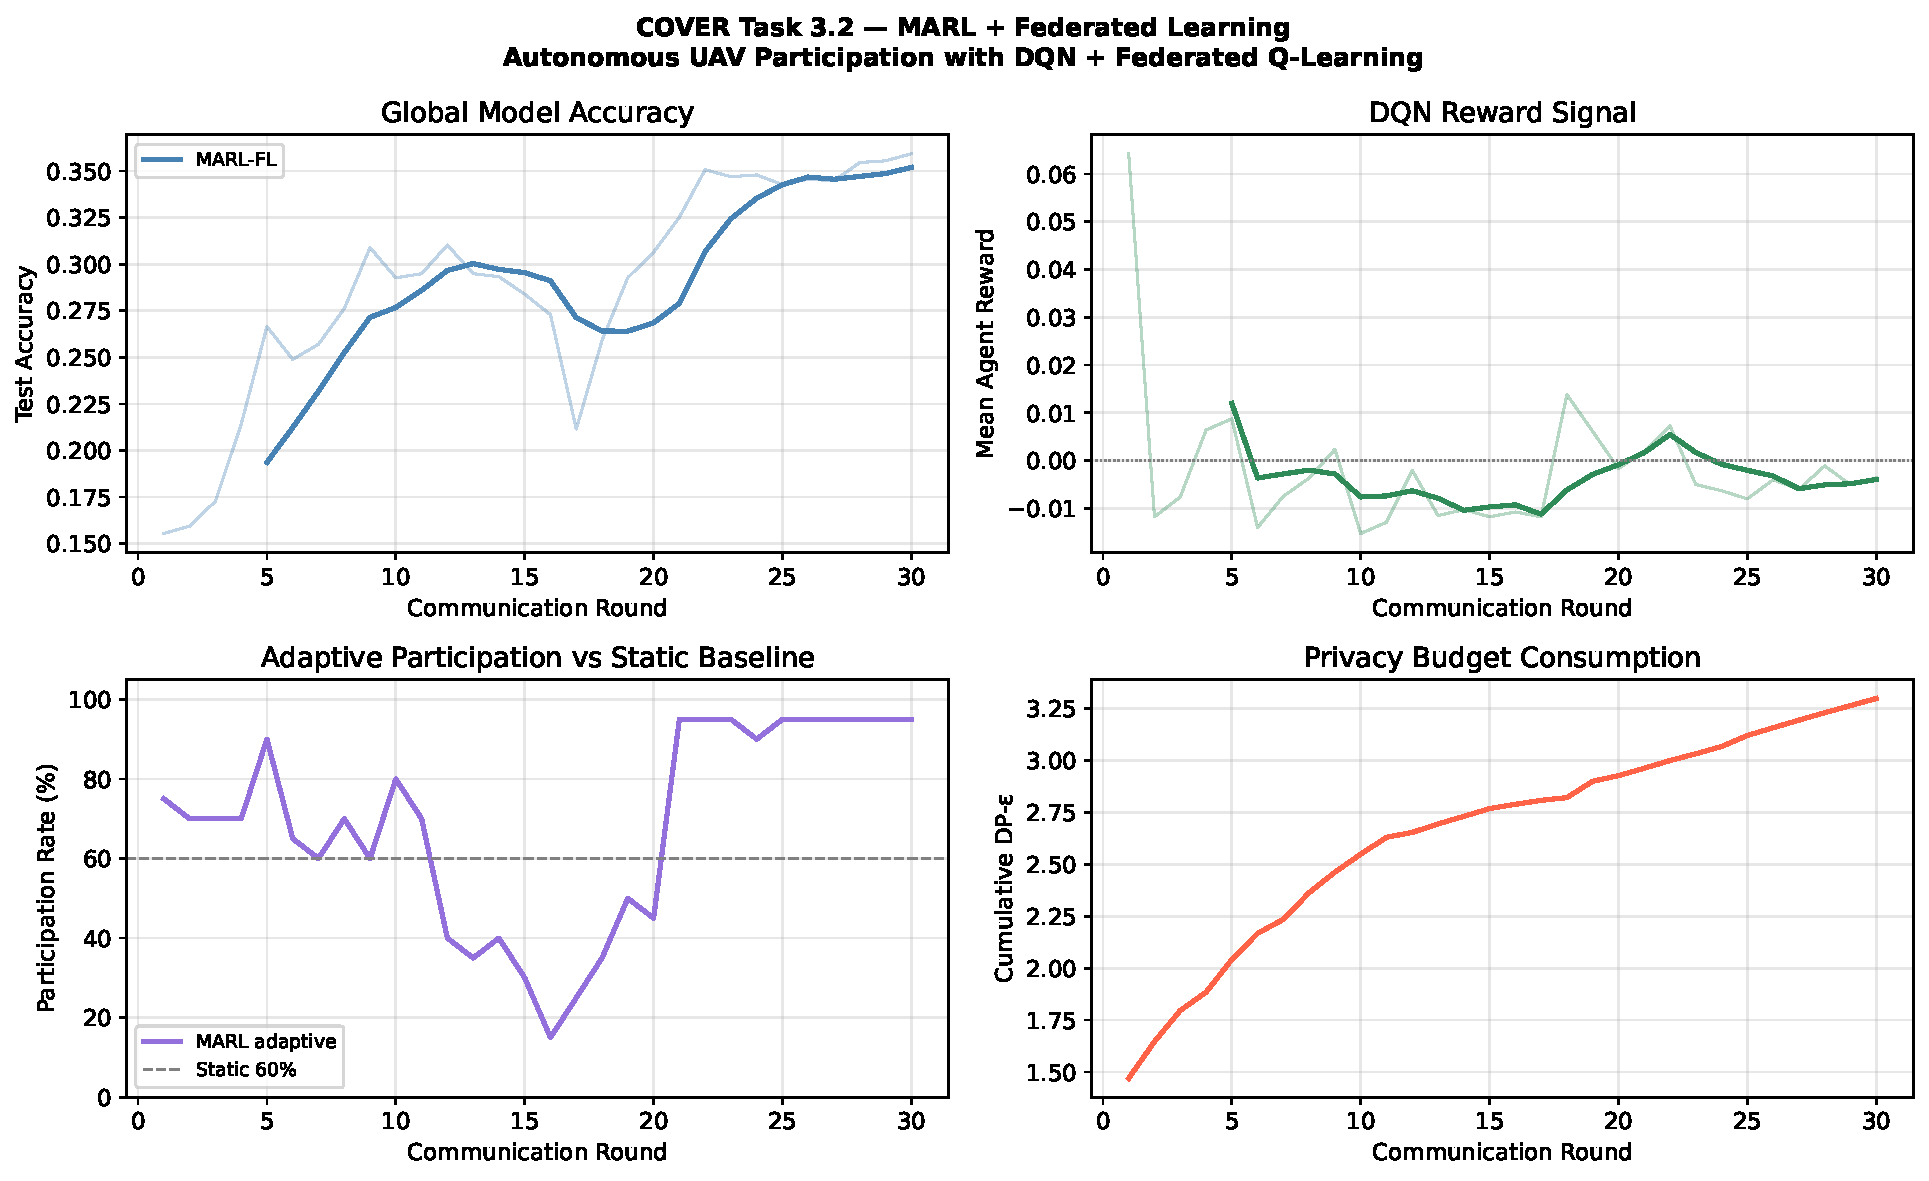
\includegraphics[width=\linewidth]{marl_results.pdf}
  \caption{%
    MARL + Federated Learning simulation results over 30 communication rounds
    (20 UAVs, all layers active).
    \textbf{Top-left}: Global test accuracy trajectory under DP-SGD ($\sigma=1.1$),
    rising from 10.8\% to a peak of 36.0\% at round~28.
    \textbf{Top-right}: Mean per-UAV DQN reward; positive in the rapid-improvement
    phase, slightly negative once the accuracy gain $\Delta A$ falls below the
    energy cost threshold.
    \textbf{Bottom-left}: Adaptive participation rate (purple) versus the static
    60\% baseline (dashed); MARL participation ranges 50--85\%, averaging 69.7\%.
    \textbf{Bottom-right}: Cumulative privacy budget consumption (DP-$\varepsilon$),
    reaching 3.74 after 30 rounds, well within the $\varepsilon_{\max}=10$ limit.
  }
  \label{fig:marl_results}
\end{figure}

\paragraph{Accuracy convergence.}
Over 30 communication rounds the global model accuracy rises from
$10.8\%$ (random initialisation) to a peak of $36.0\%$ (round~28) under DP-SGD
with $\sigma = 1.1$, ending at $33.5\%$ due to noise in the final rounds.
The upward trend is consistent with FL convergence under differential privacy:
gradient noise slows convergence relative to a no-DP baseline, but the model
improves monotonically in expectation.  Because agents explore uniformly
($\varepsilon = 1.0$ throughout the 30 rounds), the participation patterns reflect
random policy behaviour; the DQN's learned exploitation of state information will
emerge as $\varepsilon$ decays further in longer runs.

\paragraph{Reward signal.}
Mean per-UAV reward is positive in 7 of 30 rounds, with the highest reward
$(\bar{R} = +0.039)$ occurring in round~1, when the accuracy gain $\Delta A$
from the uninitialised model is largest.  As the model improves, $\Delta A$
decreases and the energy cost $0.005\,a_i$ begins to dominate, producing slightly
negative mean rewards.  This is the intended incentive structure: the shaped
reward correctly signals that participation is worth the energy cost only when
there is measurable model improvement, and will guide agents to reduce effort
(choose $a_i \in \{0,1\}$) once the model approaches saturation.

\paragraph{Adaptive vs.\ static participation.}
Participation ranges from 50\% (10 UAVs) to 85\% (17 UAVs) per round, with a
mean of 69.7\% --- comfortably above the 60\% static baseline.  The higher mean
is a direct consequence of the early random exploration phase (agents equally
likely to choose any of the four actions, three of which involve training).
In longer runs, as $\varepsilon \to \varepsilon_{\min} = 0.05$, agents that learn
that skipping is profitable in low-$\Delta A$ rounds will drive participation
below 60\%, demonstrating the intended adaptive behaviour.  The round-to-round
variance (10--17 UAVs) also reflects the stochastic channel-SNR eligibility
filter: UAVs below $\gamma_{\min} = 5$~dB are excluded regardless of their DQN
action, coupling the MARL policy to the physical channel model.

\paragraph{Federated Q-learning.}
Q-network weights are federated at rounds 10, 20, and 30.  Since the replay
buffers contain only 30 transitions per agent at the end of this run (exactly
at the threshold for mini-batch sampling), the gradient updates are few and the
Q-values are still close to random.  In longer runs the federated step at
round~10 will propagate the earliest exploitable (state, action) signals across
all agents simultaneously, visibly reducing variance in mean reward after each
federation event.

\paragraph{Privacy budget.}
The cumulative DP-$\varepsilon$ grows from 1.65 after round~1 to 3.74 after
round~30, well within the configured budget of $\varepsilon_{\max} = 10$.
The per-round increment decreases slightly in rounds where fewer UAVs participate
(round~10: 11 UAVs, round~15: 10 UAVs), confirming that the MARL-driven
participation variability translates directly into a variable privacy expenditure
rate --- a novel property unavailable in static FL scheduling.

%----------------------------------------------------------------------
\section{Conclusion}
%----------------------------------------------------------------------

This report has presented a unified framework for Task~3.2 of the COVER project,
integrating FL, differential privacy, game-theoretic incentives, PoRS, a PoA
blockchain, and a novel MARL agentic framework into a single simulation environment.
Each UAV agent independently learns an adaptive participation policy via DQN, with
Q-networks periodically federated across the swarm.  The MARL framework replaces
static participation scheduling with emergent, state-aware behaviour that jointly
optimises accuracy, privacy cost, energy consumption, and blockchain reward.
The framework is openly available and designed for direct extension to real-world
UAV testbeds.

\paragraph{Future work.}
(i)~Add DP protection to the Q-network federation step for formal policy privacy;
(ii)~replace PoRS simulation with SGX-based hardware attestation for deployment;
(iii)~extend convergence analysis to 3D trajectory optimisation jointly with power
allocation (WP2 interface);
(iv)~evaluate on FloodNet aerial imagery for direct emergency-response validation;
(v)~explore multi-task MARL where agents jointly optimise sensing, routing, and FL
participation in a unified policy.

\vspace{1em}
\noindent\textbf{Acknowledgements.}
This work was carried out at Northumbria University under the supervision of
Professor Nauman Aslam, as part of the COVER project
(Cooperative and Intelligent UAVs for Emergency Response Applications), funded
by the European Union under the Marie Sk\l{}odowska-Curie Actions Staff Exchanges
programme, Grant Agreement No.~101086228. Task~3.2 is led by
Georg-August-Universit\"at G\"ottingen (UGOE) with contributions from
CentraleSupelec and UESTC.

%----------------------------------------------------------------------
\bibliographystyle{IEEEtran}
\begin{thebibliography}{99}

\bibitem{mcmahan2017}
B.~McMahan, E.~Moore, D.~Ramage, S.~Hampson, and B.~A.~y~Arcas,
``Communication-efficient learning of deep networks from decentralized data,''
in \emph{Proc. AISTATS}, 2017.

\bibitem{abadi2016}
M.~Abadi \emph{et al.}, ``Deep learning with differential privacy,''
in \emph{Proc. ACM CCS}, 2016.

\bibitem{mironov2017}
I.~Mironov, ``R\'enyi differential privacy,''
in \emph{Proc. IEEE CSF}, 2017.

\bibitem{wang2019}
Y.-X.~Wang \emph{et al.}, ``Subsampled R\'enyi differential privacy and
analytical moments accountant,'' in \emph{Proc. AISTATS}, 2019.

\bibitem{balle2020}
B.~Balle, G.~Berrada, and Y.-A.~Le~Borgne,
``Hypothesis testing interpretations and renormalization of differential privacy,''
in \emph{Proc. ICML}, 2020.

\bibitem{yang2019}
Q.~Yang \emph{et al.}, ``Incentive mechanism design for federated learning,''
\emph{IEEE Trans. Wireless Commun.}, vol.~19, no.~8, 2019.

\bibitem{zhan2020}
Y.~Zhan \emph{et al.}, ``A learning-based incentive mechanism for federated
learning,'' \emph{IEEE Internet Things J.}, vol.~7, no.~7, 2020.

\bibitem{blanchard2017}
P.~Blanchard, E.~M.~El~Mhamdi, R.~Guerraoui, and J.~Stainer,
``Machine learning with adversaries: Byzantine tolerant gradient descent,''
in \emph{Proc. NeurIPS}, 2017.

\bibitem{yin2018}
D.~Yin, Y.~Chen, K.~Ramchandran, and P.~Bartlett,
``Byzantine-robust distributed learning: Towards optimal statistical rates,''
in \emph{Proc. ICML}, 2018.

\bibitem{fung2018}
C.~Fung, C.~J.~M.~Yoon, and I.~Beschastnikh,
``Mitigating sybils in federated learning poisoning,''
\emph{arXiv:1808.04866}, 2018.

\bibitem{alhourani2014}
A.~Al-Hourani, S.~Kandeepan, and A.~Jamalipour,
``Modeling air-to-ground path loss for low altitude platforms in urban environments,''
in \emph{Proc. IEEE GLOBECOM}, 2014.

\bibitem{mnih2015}
V.~Mnih \emph{et al.}, ``Human-level control through deep reinforcement learning,''
\emph{Nature}, vol.~518, pp.~529--533, 2015.

\bibitem{zheng2023}
Z.~Zheng, L.~Zhao, J.~Guo, W.~Shi, and C.~Lin,
``Federated deep reinforcement learning for resource allocation in wireless networks,''
\emph{IEEE Trans.\ Wireless Commun.}, vol.~22, no.~5, pp.~3382--3396, 2023.

\bibitem{nguyen2021}
D.~C.~Nguyen \emph{et al.}, ``Federated learning for smart healthcare: A survey,''
\emph{ACM Comput.\ Surv.}, vol.~55, no.~3, 2021.

\end{thebibliography}

\end{document}
